\documentclass[1p]{elsarticle_modified}
%\bibliographystyle{elsarticle-num}

%\usepackage[colorlinks]{hyperref}
%\usepackage{abbrmath_seonhwa} %\Abb, \Ascr, \Acal ,\Abf, \Afrak
\usepackage{amsfonts}
\usepackage{amssymb}
\usepackage{amsmath}
\usepackage{amsthm}
\usepackage{scalefnt}
\usepackage{amsbsy}
\usepackage{kotex}
\usepackage{caption}
\usepackage{subfig}
\usepackage{color}
\usepackage{graphicx}
\usepackage{xcolor} %% white, black, red, green, blue, cyan, magenta, yellow
\usepackage{float}
\usepackage{setspace}
\usepackage{hyperref}

\usepackage{tikz}
\usetikzlibrary{arrows}

\usepackage{multirow}
\usepackage{array} % fixed length table
\usepackage{hhline}

%%%%%%%%%%%%%%%%%%%%%
\makeatletter
\renewcommand*\env@matrix[1][\arraystretch]{%
	\edef\arraystretch{#1}%
	\hskip -\arraycolsep
	\let\@ifnextchar\new@ifnextchar
	\array{*\c@MaxMatrixCols c}}
\makeatother %https://tex.stackexchange.com/questions/14071/how-can-i-increase-the-line-spacing-in-a-matrix
%%%%%%%%%%%%%%%

\usepackage[normalem]{ulem}

\newcommand{\msout}[1]{\ifmmode\text{\sout{\ensuremath{#1}}}\else\sout{#1}\fi}
%SOURCE: \msout is \stkout macro in https://tex.stackexchange.com/questions/20609/strikeout-in-math-mode

\newcommand{\cancel}[1]{
	\ifmmode
	{\color{red}\msout{#1}}
	\else
	{\color{red}\sout{#1}}
	\fi
}

\newcommand{\add}[1]{
	{\color{blue}\uwave{#1}}
}

\newcommand{\replace}[2]{
	\ifmmode
	{\color{red}\msout{#1}}{\color{blue}\uwave{#2}}
	\else
	{\color{red}\sout{#1}}{\color{blue}\uwave{#2}}
	\fi
}

\newcommand{\Sol}{\mathcal{S}} %segment
\newcommand{\D}{D} %diagram
\newcommand{\A}{\mathcal{A}} %arc


%%%%%%%%%%%%%%%%%%%%%%%%%%%%%5 test

\def\sl{\operatorname{\textup{SL}}(2,\Cbb)}
\def\psl{\operatorname{\textup{PSL}}(2,\Cbb)}
\def\quan{\mkern 1mu \triangleright \mkern 1mu}

\theoremstyle{definition}
\newtheorem{thm}{Theorem}[section]
\newtheorem{prop}[thm]{Proposition}
\newtheorem{lem}[thm]{Lemma}
\newtheorem{ques}[thm]{Question}
\newtheorem{cor}[thm]{Corollary}
\newtheorem{defn}[thm]{Definition}
\newtheorem{exam}[thm]{Example}
\newtheorem{rmk}[thm]{Remark}
\newtheorem{alg}[thm]{Algorithm}

\newcommand{\I}{\sqrt{-1}}
\begin{document}

%\begin{frontmatter}
%
%\title{Boundary parabolic representations of knots up to 8 crossings}
%
%%% Group authors per affiliation:
%\author{Yunhi Cho} 
%\address{Department of Mathematics, University of Seoul, Seoul, Korea}
%\ead{yhcho@uos.ac.kr}
%
%
%\author{Seonhwa Kim} %\fnref{s_kim}}
%\address{Center for Geometry and Physics, Institute for Basic Science, Pohang, 37673, Korea}
%\ead{ryeona17@ibs.re.kr}
%
%\author{Hyuk Kim}
%\address{Department of Mathematical Sciences, Seoul National University, Seoul 08826, Korea}
%\ead{hyukkim@snu.ac.kr}
%
%\author{Seokbeom Yoon}
%\address{Department of Mathematical Sciences, Seoul National University, Seoul, 08826,  Korea}
%\ead{sbyoon15@snu.ac.kr}
%
%\begin{abstract}
%We find all boundary parabolic representation of knots up to 8 crossings.
%
%\end{abstract}
%\begin{keyword}
%    \MSC[2010] 57M25 
%\end{keyword}
%
%\end{frontmatter}

%\linenumbers
%\tableofcontents
%
\newcommand\colored[1]{\textcolor{white}{\rule[-0.35ex]{0.8em}{1.4ex}}\kern-0.8em\color{red} #1}%
%\newcommand\colored[1]{\textcolor{white}{ #1}\kern-2.17ex	\textcolor{white}{ #1}\kern-1.81ex	\textcolor{white}{ #1}\kern-2.15ex\color{red}#1	}

{\Large $\underline{12a_{0156}~(K12a_{0156})}$}

\setlength{\tabcolsep}{10pt}
\renewcommand{\arraystretch}{1.6}
\vspace{1cm}\begin{tabular}{m{100pt}>{\centering\arraybackslash}m{274pt}}
\multirow{5}{120pt}{
	\centering
	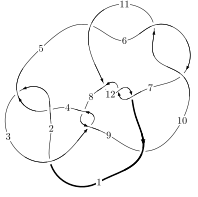
\includegraphics[width=112pt]{../../../GIT/diagram.site/Diagrams/png/957_12a_0156.png}\\
\ \ \ A knot diagram\footnotemark}&
\allowdisplaybreaks
\textbf{Linearized knot diagam} \\
\cline{2-2}
 &
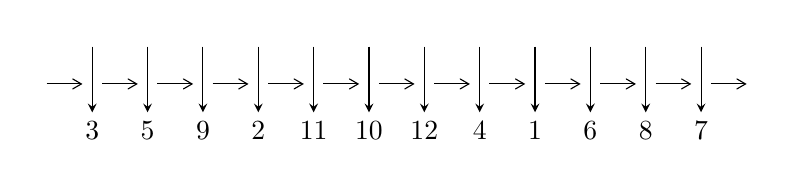
\begin{tikzpicture}[x=20pt, y=17pt]
	% nodes
	\node (C0) at (0, 0) {};
	\node (C1) at (1, 0) {};
	\node (C1U) at (1, +1) {};
	\node (C1D) at (1, -1) {3};

	\node (C2) at (2, 0) {};
	\node (C2U) at (2, +1) {};
	\node (C2D) at (2, -1) {5};

	\node (C3) at (3, 0) {};
	\node (C3U) at (3, +1) {};
	\node (C3D) at (3, -1) {9};

	\node (C4) at (4, 0) {};
	\node (C4U) at (4, +1) {};
	\node (C4D) at (4, -1) {2};

	\node (C5) at (5, 0) {};
	\node (C5U) at (5, +1) {};
	\node (C5D) at (5, -1) {11};

	\node (C6) at (6, 0) {};
	\node (C6U) at (6, +1) {};
	\node (C6D) at (6, -1) {10};

	\node (C7) at (7, 0) {};
	\node (C7U) at (7, +1) {};
	\node (C7D) at (7, -1) {12};

	\node (C8) at (8, 0) {};
	\node (C8U) at (8, +1) {};
	\node (C8D) at (8, -1) {4};

	\node (C9) at (9, 0) {};
	\node (C9U) at (9, +1) {};
	\node (C9D) at (9, -1) {1};

	\node (C10) at (10, 0) {};
	\node (C10U) at (10, +1) {};
	\node (C10D) at (10, -1) {6};

	\node (C11) at (11, 0) {};
	\node (C11U) at (11, +1) {};
	\node (C11D) at (11, -1) {8};

	\node (C12) at (12, 0) {};
	\node (C12U) at (12, +1) {};
	\node (C12D) at (12, -1) {7};
	\node (C13) at (13, 0) {};

	% arrows
	\draw[->,>={angle 60}]
	(C0) edge (C1) (C1) edge (C2) (C2) edge (C3) (C3) edge (C4) (C4) edge (C5) (C5) edge (C6) (C6) edge (C7) (C7) edge (C8) (C8) edge (C9) (C9) edge (C10) (C10) edge (C11) (C11) edge (C12) (C12) edge (C13) ;	\draw[->,>=stealth]
	(C1U) edge (C1D) (C2U) edge (C2D) (C3U) edge (C3D) (C4U) edge (C4D) (C5U) edge (C5D) (C6U) edge (C6D) (C7U) edge (C7D) (C8U) edge (C8D) (C9U) edge (C9D) (C10U) edge (C10D) (C11U) edge (C11D) (C12U) edge (C12D) ;
	\end{tikzpicture} \\
\hhline{~~} \\& 
\textbf{Solving Sequence} \\ \cline{2-2} 
 &
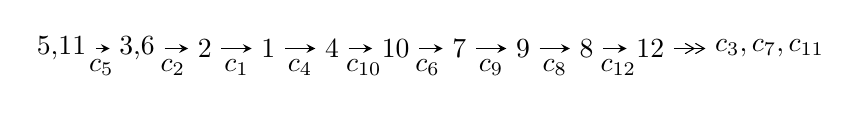
\begin{tikzpicture}[x=23pt, y=7pt]
	% node
	\node (A0) at (-1/8, 0) {5,11};
	\node (A1) at (17/16, 0) {3,6};
	\node (A2) at (17/8, 0) {2};
	\node (A3) at (25/8, 0) {1};
	\node (A4) at (33/8, 0) {4};
	\node (A5) at (41/8, 0) {10};
	\node (A6) at (49/8, 0) {7};
	\node (A7) at (57/8, 0) {9};
	\node (A8) at (65/8, 0) {8};
	\node (A9) at (73/8, 0) {12};
	\node (C1) at (1/2, -1) {$c_{5}$};
	\node (C2) at (13/8, -1) {$c_{2}$};
	\node (C3) at (21/8, -1) {$c_{1}$};
	\node (C4) at (29/8, -1) {$c_{4}$};
	\node (C5) at (37/8, -1) {$c_{10}$};
	\node (C6) at (45/8, -1) {$c_{6}$};
	\node (C7) at (53/8, -1) {$c_{9}$};
	\node (C8) at (61/8, -1) {$c_{8}$};
	\node (C9) at (69/8, -1) {$c_{12}$};
	\node (A10) at (11, 0) {$c_{3},c_{7},c_{11}$};

	% edge
	\draw[->,>=stealth]	
	(A0) edge (A1) (A1) edge (A2) (A2) edge (A3) (A3) edge (A4) (A4) edge (A5) (A5) edge (A6) (A6) edge (A7) (A7) edge (A8) (A8) edge (A9) ;
	\draw[->>,>={angle 60}]	
	(A9) edge (A10);
\end{tikzpicture} \\ 

\end{tabular} \\

\footnotetext{
The image of knot diagram is generated by the software ``\textbf{Draw programme}" developed by Andrew Bartholomew(\url{http://www.layer8.co.uk/maths/draw/index.htm\#Running-draw}), where we modified some parts for our purpose(\url{https://github.com/CATsTAILs/LinksPainter}).
}\phantom \\ \newline 
\centering \textbf{Ideals for irreducible components\footnotemark of $X_{\text{par}}$} 
 
\begin{align*}
I^u_{1}&=\langle 
3 u^{38}-51 u^{37}+\cdots+256 b-85,\;-121 u^{38}+133 u^{37}+\cdots+512 a-61,\;u^{39}+25 u^{37}+\cdots+u+1\rangle \\
I^u_{2}&=\langle 
2.94986\times10^{44} u^{49}+3.65735\times10^{44} u^{48}+\cdots+2.95826\times10^{45} b-1.68829\times10^{45},\\
\phantom{I^u_{2}}&\phantom{= \langle  }2.14090\times10^{45} u^{49}+1.60923\times10^{45} u^{48}+\cdots+8.87477\times10^{45} a-4.58714\times10^{45},\;u^{50}+2 u^{49}+\cdots-18 u+9\rangle \\
I^u_{3}&=\langle 
-54276 a^5 u+156246 a^4 u+\cdots+839054 a-188617,\\
\phantom{I^u_{3}}&\phantom{= \langle  }a^6+2 a^5 u-4 a^4 u- a^4+4 a^3 u+6 a^3+a^2 u+4 a^2+10 a u+a+4 u-1,\;u^2+1\rangle \\
I^u_{4}&=\langle 
b+1,\;u^2+2 a+u+3,\;u^3+2 u-1\rangle \\
I^u_{5}&=\langle 
b+1,\;u^3+u^2+a+u+2,\;u^4+u^3+2 u^2+2 u+1\rangle \\
\\
\end{align*}
\raggedright * 5 irreducible components of $\dim_{\mathbb{C}}=0$, with total 108 representations.\\
\footnotetext{All coefficients of polynomials are rational numbers. But the coefficients are sometimes approximated in decimal forms when there is not enough margin.}
\newpage
\renewcommand{\arraystretch}{1}
\centering \section*{I. $I^u_{1}= \langle 3 u^{38}-51 u^{37}+\cdots+256 b-85,\;-121 u^{38}+133 u^{37}+\cdots+512 a-61,\;u^{39}+25 u^{37}+\cdots+u+1 \rangle$}
\flushleft \textbf{(i) Arc colorings}\\
\begin{tabular}{m{7pt} m{180pt} m{7pt} m{180pt} }
\flushright $a_{5}=$&$\begin{pmatrix}1\\0\end{pmatrix}$ \\
\flushright $a_{11}=$&$\begin{pmatrix}0\\u\end{pmatrix}$ \\
\flushright $a_{3}=$&$\begin{pmatrix}0.236328 u^{38}-0.259766 u^{37}+\cdots-0.976563 u+0.119141\\-0.0117188 u^{38}+0.199219 u^{37}+\cdots+1.71875 u+0.332031\end{pmatrix}$ \\
\flushright $a_{6}=$&$\begin{pmatrix}1\\u^2\end{pmatrix}$ \\
\flushright $a_{2}=$&$\begin{pmatrix}0.224609 u^{38}-0.0605469 u^{37}+\cdots+0.742188 u+0.451172\\-0.0117188 u^{38}+0.199219 u^{37}+\cdots+1.71875 u+0.332031\end{pmatrix}$ \\
\flushright $a_{1}=$&$\begin{pmatrix}- u^3-2 u\\\frac{1}{64} u^{38}+\frac{3}{8} u^{36}+\cdots+\frac{1}{64} u^2+\frac{65}{64} u\end{pmatrix}$ \\
\flushright $a_{4}=$&$\begin{pmatrix}0.0878906 u^{38}-0.0644531 u^{37}+\cdots+1.07031 u+1.04883\\-0.199219 u^{38}-0.207031 u^{37}+\cdots-1.50000 u-0.761719\end{pmatrix}$ \\
\flushright $a_{10}=$&$\begin{pmatrix}u\\u^3+u\end{pmatrix}$ \\
\flushright $a_{7}=$&$\begin{pmatrix}u^2+1\\u^4+2 u^2\end{pmatrix}$ \\
\flushright $a_{9}=$&$\begin{pmatrix}-0.0156250 u^{38}-0.375000 u^{36}+\cdots-0.0156250 u^{2}+0.984375 u\\0.0312500 u^{38}+0.0312500 u^{37}+\cdots+1.09375 u+0.0312500\end{pmatrix}$ \\
\flushright $a_{8}=$&$\begin{pmatrix}-1\\\frac{1}{64} u^{37}+\frac{3}{8} u^{35}+\cdots+\frac{1}{64} u+\frac{1}{64}\end{pmatrix}$ \\
\flushright $a_{12}=$&$\begin{pmatrix}- u\\\frac{1}{64} u^{38}+\frac{3}{8} u^{36}+\cdots+\frac{1}{64} u^2+\frac{65}{64} u\end{pmatrix}$\\&\end{tabular}
\flushleft \textbf{(ii) Obstruction class $= -1$}\\~\\
\flushleft \textbf{(iii) Cusp Shapes $= -\frac{2567}{1024} u^{38}+\frac{507}{1024} u^{37}+\cdots+\frac{2683}{256} u-\frac{8131}{1024}$}\\~\\
\newpage\renewcommand{\arraystretch}{1}
\flushleft \textbf{(iv) u-Polynomials at the component}\newline \\
\begin{tabular}{m{50pt}|m{274pt}}
Crossings & \hspace{64pt}u-Polynomials at each crossing \\
\hline $$\begin{aligned}c_{1}\end{aligned}$$&$\begin{aligned}
&u^{39}+18 u^{38}+\cdots+817 u+16
\end{aligned}$\\
\hline $$\begin{aligned}c_{2},c_{4}\end{aligned}$$&$\begin{aligned}
&u^{39}-4 u^{38}+\cdots+13 u+4
\end{aligned}$\\
\hline $$\begin{aligned}c_{3},c_{8}\end{aligned}$$&$\begin{aligned}
&u^{39}-3 u^{38}+\cdots-8 u+32
\end{aligned}$\\
\hline $$\begin{aligned}c_{5},c_{6},c_{7}\\c_{10},c_{11},c_{12}\end{aligned}$$&$\begin{aligned}
&u^{39}+25 u^{37}+\cdots+u+1
\end{aligned}$\\
\hline $$\begin{aligned}c_{9}\end{aligned}$$&$\begin{aligned}
&u^{39}+24 u^{38}+\cdots+132148 u+10276
\end{aligned}$\\
\hline
\end{tabular}\\~\\
\newpage\renewcommand{\arraystretch}{1}
\flushleft \textbf{(v) Riley Polynomials at the component}\newline \\
\begin{tabular}{m{50pt}|m{274pt}}
Crossings & \hspace{64pt}Riley Polynomials at each crossing \\
\hline $$\begin{aligned}c_{1}\end{aligned}$$&$\begin{aligned}
&y^{39}+10 y^{38}+\cdots+507201 y-256
\end{aligned}$\\
\hline $$\begin{aligned}c_{2},c_{4}\end{aligned}$$&$\begin{aligned}
&y^{39}-18 y^{38}+\cdots+817 y-16
\end{aligned}$\\
\hline $$\begin{aligned}c_{3},c_{8}\end{aligned}$$&$\begin{aligned}
&y^{39}+21 y^{38}+\cdots-3776 y-1024
\end{aligned}$\\
\hline $$\begin{aligned}c_{5},c_{6},c_{7}\\c_{10},c_{11},c_{12}\end{aligned}$$&$\begin{aligned}
&y^{39}+50 y^{38}+\cdots-3 y-1
\end{aligned}$\\
\hline $$\begin{aligned}c_{9}\end{aligned}$$&$\begin{aligned}
&y^{39}+18 y^{38}+\cdots-277125320 y-105596176
\end{aligned}$\\
\hline
\end{tabular}\\~\\
\newpage\flushleft \textbf{(vi) Complex Volumes and Cusp Shapes}
$$\begin{array}{c|c|c}  
\text{Solutions to }I^u_{1}& \I (\text{vol} + \sqrt{-1}CS) & \text{Cusp shape}\\
 \hline 
\begin{aligned}
u &= \phantom{-}0.606138 + 0.433746 I \\
a &= \phantom{-}1.10839 - 1.72999 I \\
b &= \phantom{-}1.096070 + 0.636892 I\end{aligned}
 & \phantom{-}1.24768 - 8.38959 I & -11.7192 + 9.4891 I \\ \hline\begin{aligned}
u &= \phantom{-}0.606138 - 0.433746 I \\
a &= \phantom{-}1.10839 + 1.72999 I \\
b &= \phantom{-}1.096070 - 0.636892 I\end{aligned}
 & \phantom{-}1.24768 + 8.38959 I & -11.7192 - 9.4891 I \\ \hline\begin{aligned}
u &= -0.686742 + 0.093387 I \\
a &= \phantom{-}1.124820 + 0.357401 I \\
b &= \phantom{-}0.888553 + 0.474189 I\end{aligned}
 & -1.46543 - 1.90675 I & -13.8759 + 2.9903 I \\ \hline\begin{aligned}
u &= -0.686742 - 0.093387 I \\
a &= \phantom{-}1.124820 - 0.357401 I \\
b &= \phantom{-}0.888553 - 0.474189 I\end{aligned}
 & -1.46543 + 1.90675 I & -13.8759 - 2.9903 I \\ \hline\begin{aligned}
u &= \phantom{-}0.512624 + 0.450918 I \\
a &= -0.817372 + 0.180228 I \\
b &= \phantom{-}0.464938 - 0.809663 I\end{aligned}
 & \phantom{-}3.12365 - 2.96834 I & -8.53439 + 5.45411 I \\ \hline\begin{aligned}
u &= \phantom{-}0.512624 - 0.450918 I \\
a &= -0.817372 - 0.180228 I \\
b &= \phantom{-}0.464938 + 0.809663 I\end{aligned}
 & \phantom{-}3.12365 + 2.96834 I & -8.53439 - 5.45411 I \\ \hline\begin{aligned}
u &= \phantom{-}0.097297 + 1.396560 I \\
a &= \phantom{-}0.600483 - 0.695228 I \\
b &= \phantom{-}1.132180 + 0.452280 I\end{aligned}
 & \phantom{-}5.93701 - 6.97505 I & \phantom{-0.000000 } 0 \\ \hline\begin{aligned}
u &= \phantom{-}0.097297 - 1.396560 I \\
a &= \phantom{-}0.600483 + 0.695228 I \\
b &= \phantom{-}1.132180 - 0.452280 I\end{aligned}
 & \phantom{-}5.93701 + 6.97505 I & \phantom{-0.000000 } 0 \\ \hline\begin{aligned}
u &= -0.485730 + 0.337100 I \\
a &= -0.58443 - 2.43918 I \\
b &= -0.928433 + 0.452438 I\end{aligned}
 & -1.46092 + 2.88558 I & -14.3616 - 7.5955 I \\ \hline\begin{aligned}
u &= -0.485730 - 0.337100 I \\
a &= -0.58443 + 2.43918 I \\
b &= -0.928433 - 0.452438 I\end{aligned}
 & -1.46092 - 2.88558 I & -14.3616 + 7.5955 I\\
 \hline 
 \end{array}$$\newpage$$\begin{array}{c|c|c}  
\text{Solutions to }I^u_{1}& \I (\text{vol} + \sqrt{-1}CS) & \text{Cusp shape}\\
 \hline 
\begin{aligned}
u &= \phantom{-}0.160047 + 0.560104 I \\
a &= -0.472825 + 0.884195 I \\
b &= \phantom{-}1.058660 - 0.598292 I\end{aligned}
 & \phantom{-}1.75331 + 5.17154 I & -10.85539 - 2.38918 I \\ \hline\begin{aligned}
u &= \phantom{-}0.160047 - 0.560104 I \\
a &= -0.472825 - 0.884195 I \\
b &= \phantom{-}1.058660 + 0.598292 I\end{aligned}
 & \phantom{-}1.75331 - 5.17154 I & -10.85539 + 2.38918 I \\ \hline\begin{aligned}
u &= \phantom{-}0.255669 + 0.512819 I \\
a &= \phantom{-}0.095335 - 1.276560 I \\
b &= \phantom{-}0.500188 + 0.744588 I\end{aligned}
 & \phantom{-}3.42355 + 0.06447 I & -7.35584 + 3.68014 I \\ \hline\begin{aligned}
u &= \phantom{-}0.255669 - 0.512819 I \\
a &= \phantom{-}0.095335 + 1.276560 I \\
b &= \phantom{-}0.500188 - 0.744588 I\end{aligned}
 & \phantom{-}3.42355 - 0.06447 I & -7.35584 - 3.68014 I \\ \hline\begin{aligned}
u &= \phantom{-}0.24730 + 1.43914 I \\
a &= \phantom{-}0.342403 - 0.242192 I \\
b &= \phantom{-}0.835724 - 0.187359 I\end{aligned}
 & \phantom{-}8.20195 - 4.67633 I & \phantom{-0.000000 } 0 \\ \hline\begin{aligned}
u &= \phantom{-}0.24730 - 1.43914 I \\
a &= \phantom{-}0.342403 + 0.242192 I \\
b &= \phantom{-}0.835724 + 0.187359 I\end{aligned}
 & \phantom{-}8.20195 + 4.67633 I & \phantom{-0.000000 } 0 \\ \hline\begin{aligned}
u &= -0.01911 + 1.46623 I \\
a &= -0.513457 - 0.986167 I \\
b &= -1.218970 + 0.402466 I\end{aligned}
 & \phantom{-}5.58893 + 1.41780 I & \phantom{-0.000000 } 0 \\ \hline\begin{aligned}
u &= -0.01911 - 1.46623 I \\
a &= -0.513457 + 0.986167 I \\
b &= -1.218970 - 0.402466 I\end{aligned}
 & \phantom{-}5.58893 - 1.41780 I & \phantom{-0.000000 } 0 \\ \hline\begin{aligned}
u &= \phantom{-}0.07057 + 1.49185 I \\
a &= \phantom{-}0.206418 + 0.688633 I \\
b &= -0.036484 - 0.767123 I\end{aligned}
 & \phantom{-}9.22311 - 2.89697 I & \phantom{-0.000000 } 0 \\ \hline\begin{aligned}
u &= \phantom{-}0.07057 - 1.49185 I \\
a &= \phantom{-}0.206418 - 0.688633 I \\
b &= -0.036484 + 0.767123 I\end{aligned}
 & \phantom{-}9.22311 + 2.89697 I & \phantom{-0.000000 } 0\\
 \hline 
 \end{array}$$\newpage$$\begin{array}{c|c|c}  
\text{Solutions to }I^u_{1}& \I (\text{vol} + \sqrt{-1}CS) & \text{Cusp shape}\\
 \hline 
\begin{aligned}
u &= \phantom{-}0.435690 + 0.236154 I \\
a &= -1.49896 + 0.88737 I \\
b &= -1.166600 + 0.114063 I\end{aligned}
 & -2.34640 - 0.81341 I & -13.1026 + 8.4479 I \\ \hline\begin{aligned}
u &= \phantom{-}0.435690 - 0.236154 I \\
a &= -1.49896 - 0.88737 I \\
b &= -1.166600 - 0.114063 I\end{aligned}
 & -2.34640 + 0.81341 I & -13.1026 - 8.4479 I \\ \hline\begin{aligned}
u &= -0.27417 + 1.55715 I \\
a &= -0.099646 - 0.449882 I \\
b &= -1.372790 - 0.112918 I\end{aligned}
 & \phantom{-}10.02810 + 6.61870 I & \phantom{-0.000000 } 0 \\ \hline\begin{aligned}
u &= -0.27417 - 1.55715 I \\
a &= -0.099646 + 0.449882 I \\
b &= -1.372790 + 0.112918 I\end{aligned}
 & \phantom{-}10.02810 - 6.61870 I & \phantom{-0.000000 } 0 \\ \hline\begin{aligned}
u &= \phantom{-}0.30186 + 1.56039 I \\
a &= \phantom{-}0.02339 + 2.01745 I \\
b &= -0.977777 - 0.644002 I\end{aligned}
 & \phantom{-}11.2737 - 9.4013 I & \phantom{-0.000000 } 0 \\ \hline\begin{aligned}
u &= \phantom{-}0.30186 - 1.56039 I \\
a &= \phantom{-}0.02339 - 2.01745 I \\
b &= -0.977777 + 0.644002 I\end{aligned}
 & \phantom{-}11.2737 + 9.4013 I & \phantom{-0.000000 } 0 \\ \hline\begin{aligned}
u &= -0.35789 + 1.55459 I \\
a &= \phantom{-}0.37718 + 1.87847 I \\
b &= \phantom{-}1.184010 - 0.683858 I\end{aligned}
 & \phantom{-}14.1914 + 16.2242 I & \phantom{-0.000000 } 0 \\ \hline\begin{aligned}
u &= -0.35789 - 1.55459 I \\
a &= \phantom{-}0.37718 - 1.87847 I \\
b &= \phantom{-}1.184010 + 0.683858 I\end{aligned}
 & \phantom{-}14.1914 - 16.2242 I & \phantom{-0.000000 } 0 \\ \hline\begin{aligned}
u &= \phantom{-}0.24560 + 1.57817 I \\
a &= \phantom{-}0.94180 - 1.09265 I \\
b &= -0.684865 + 0.701681 I\end{aligned}
 & \phantom{-}12.16600 - 4.21253 I & \phantom{-0.000000 } 0 \\ \hline\begin{aligned}
u &= \phantom{-}0.24560 - 1.57817 I \\
a &= \phantom{-}0.94180 + 1.09265 I \\
b &= -0.684865 - 0.701681 I\end{aligned}
 & \phantom{-}12.16600 + 4.21253 I & \phantom{-0.000000 } 0\\
 \hline 
 \end{array}$$\newpage$$\begin{array}{c|c|c}  
\text{Solutions to }I^u_{1}& \I (\text{vol} + \sqrt{-1}CS) & \text{Cusp shape}\\
 \hline 
\begin{aligned}
u &= -0.198432 + 0.335342 I \\
a &= \phantom{-}1.51348 + 1.09795 I \\
b &= -0.837871 - 0.313169 I\end{aligned}
 & -0.884650 - 0.467058 I & -11.90822 - 2.02853 I \\ \hline\begin{aligned}
u &= -0.198432 - 0.335342 I \\
a &= \phantom{-}1.51348 - 1.09795 I \\
b &= -0.837871 + 0.313169 I\end{aligned}
 & -0.884650 + 0.467058 I & -11.90822 + 2.02853 I \\ \hline\begin{aligned}
u &= -0.33367 + 1.57837 I \\
a &= -0.848602 - 0.806276 I \\
b &= \phantom{-}0.422675 + 0.993588 I\end{aligned}
 & \phantom{-}16.5334 + 10.1404 I & \phantom{-0.000000 } 0 \\ \hline\begin{aligned}
u &= -0.33367 - 1.57837 I \\
a &= -0.848602 + 0.806276 I \\
b &= \phantom{-}0.422675 - 0.993588 I\end{aligned}
 & \phantom{-}16.5334 - 10.1404 I & \phantom{-0.000000 } 0 \\ \hline\begin{aligned}
u &= -0.22952 + 1.64191 I \\
a &= -0.17339 + 1.41527 I \\
b &= \phantom{-}0.671373 - 0.949740 I\end{aligned}
 & \phantom{-}18.2436 + 4.6595 I & \phantom{-0.000000 } 0 \\ \hline\begin{aligned}
u &= -0.22952 - 1.64191 I \\
a &= -0.17339 - 1.41527 I \\
b &= \phantom{-}0.671373 + 0.949740 I\end{aligned}
 & \phantom{-}18.2436 - 4.6595 I & \phantom{-0.000000 } 0 \\ \hline\begin{aligned}
u &= -0.340813\phantom{ +0.000000I} \\
a &= \phantom{-}0.891121\phantom{ +0.000000I} \\
b &= -0.149888\phantom{ +0.000000I}\end{aligned}
 & -0.576114\phantom{ +0.000000I} & -17.1030\phantom{ +0.000000I} \\ \hline\begin{aligned}
u &= -0.17712 + 1.65299 I \\
a &= -0.520565 - 1.116590 I \\
b &= \phantom{-}1.044360 + 0.795151 I\end{aligned}
 & \phantom{-}17.1048 - 1.6856 I & \phantom{-0.000000 } 0 \\ \hline\begin{aligned}
u &= -0.17712 - 1.65299 I \\
a &= -0.520565 + 1.116590 I \\
b &= \phantom{-}1.044360 - 0.795151 I\end{aligned}
 & \phantom{-}17.1048 + 1.6856 I & \phantom{-0.000000 } 0\\
 \hline 
 \end{array}$$\newpage\newpage\renewcommand{\arraystretch}{1}
\centering \section*{II. $I^u_{2}= \langle 2.95\times10^{44} u^{49}+3.66\times10^{44} u^{48}+\cdots+2.96\times10^{45} b-1.69\times10^{45},\;2.14\times10^{45} u^{49}+1.61\times10^{45} u^{48}+\cdots+8.87\times10^{45} a-4.59\times10^{45},\;u^{50}+2 u^{49}+\cdots-18 u+9 \rangle$}
\flushleft \textbf{(i) Arc colorings}\\
\begin{tabular}{m{7pt} m{180pt} m{7pt} m{180pt} }
\flushright $a_{5}=$&$\begin{pmatrix}1\\0\end{pmatrix}$ \\
\flushright $a_{11}=$&$\begin{pmatrix}0\\u\end{pmatrix}$ \\
\flushright $a_{3}=$&$\begin{pmatrix}-0.241234 u^{49}-0.181326 u^{48}+\cdots+0.375683 u+0.516874\\-0.0997162 u^{49}-0.123632 u^{48}+\cdots+0.184639 u+0.570706\end{pmatrix}$ \\
\flushright $a_{6}=$&$\begin{pmatrix}1\\u^2\end{pmatrix}$ \\
\flushright $a_{2}=$&$\begin{pmatrix}-0.340950 u^{49}-0.304958 u^{48}+\cdots+0.560322 u+1.08758\\-0.0997162 u^{49}-0.123632 u^{48}+\cdots+0.184639 u+0.570706\end{pmatrix}$ \\
\flushright $a_{1}=$&$\begin{pmatrix}-0.196743 u^{49}-0.293319 u^{48}+\cdots-13.0617 u+2.90182\\-0.0474075 u^{49}-0.0235454 u^{48}+\cdots-3.48640 u+0.424677\end{pmatrix}$ \\
\flushright $a_{4}=$&$\begin{pmatrix}-0.0231020 u^{49}+0.328429 u^{48}+\cdots+9.25365 u-3.09937\\0.0273358 u^{49}+0.145463 u^{48}+\cdots+1.17016 u-1.26078\end{pmatrix}$ \\
\flushright $a_{10}=$&$\begin{pmatrix}u\\u^3+u\end{pmatrix}$ \\
\flushright $a_{7}=$&$\begin{pmatrix}u^2+1\\u^4+2 u^2\end{pmatrix}$ \\
\flushright $a_{9}=$&$\begin{pmatrix}-0.137409 u^{49}-0.303786 u^{48}+\cdots-5.99590 u+2.47777\\-0.0865588 u^{49}-0.101282 u^{48}+\cdots-1.77113 u+0.685381\end{pmatrix}$ \\
\flushright $a_{8}=$&$\begin{pmatrix}0.0471513 u^{49}+0.147673 u^{48}+\cdots-7.45718 u+4.92740\\-0.100202 u^{49}-0.286035 u^{48}+\cdots+0.536308 u+0.519665\end{pmatrix}$ \\
\flushright $a_{12}=$&$\begin{pmatrix}-0.164482 u^{49}-0.228762 u^{48}+\cdots-16.5539 u+2.42436\\0.0322612 u^{49}+0.0645573 u^{48}+\cdots-1.49216 u-0.477454\end{pmatrix}$\\&\end{tabular}
\flushleft \textbf{(ii) Obstruction class $= -1$}\\~\\
\flushleft \textbf{(iii) Cusp Shapes $= -0.817749 u^{49}-1.70803 u^{48}+\cdots-1.83623 u-9.61323$}\\~\\
\newpage\renewcommand{\arraystretch}{1}
\flushleft \textbf{(iv) u-Polynomials at the component}\newline \\
\begin{tabular}{m{50pt}|m{274pt}}
Crossings & \hspace{64pt}u-Polynomials at each crossing \\
\hline $$\begin{aligned}c_{1}\end{aligned}$$&$\begin{aligned}
&(u^{25}+11 u^{24}+\cdots-2 u+1)^{2}
\end{aligned}$\\
\hline $$\begin{aligned}c_{2},c_{4}\end{aligned}$$&$\begin{aligned}
&(u^{25}-3 u^{24}+\cdots-4 u+1)^{2}
\end{aligned}$\\
\hline $$\begin{aligned}c_{3},c_{8}\end{aligned}$$&$\begin{aligned}
&(u^{25}+u^{24}+\cdots+4 u-4)^{2}
\end{aligned}$\\
\hline $$\begin{aligned}c_{5},c_{6},c_{7}\\c_{10},c_{11},c_{12}\end{aligned}$$&$\begin{aligned}
&u^{50}+2 u^{49}+\cdots-18 u+9
\end{aligned}$\\
\hline $$\begin{aligned}c_{9}\end{aligned}$$&$\begin{aligned}
&(u^{25}-8 u^{24}+\cdots+11 u+1)^{2}
\end{aligned}$\\
\hline
\end{tabular}\\~\\
\newpage\renewcommand{\arraystretch}{1}
\flushleft \textbf{(v) Riley Polynomials at the component}\newline \\
\begin{tabular}{m{50pt}|m{274pt}}
Crossings & \hspace{64pt}Riley Polynomials at each crossing \\
\hline $$\begin{aligned}c_{1}\end{aligned}$$&$\begin{aligned}
&(y^{25}+9 y^{24}+\cdots-2 y-1)^{2}
\end{aligned}$\\
\hline $$\begin{aligned}c_{2},c_{4}\end{aligned}$$&$\begin{aligned}
&(y^{25}-11 y^{24}+\cdots-2 y-1)^{2}
\end{aligned}$\\
\hline $$\begin{aligned}c_{3},c_{8}\end{aligned}$$&$\begin{aligned}
&(y^{25}+15 y^{24}+\cdots-88 y-16)^{2}
\end{aligned}$\\
\hline $$\begin{aligned}c_{5},c_{6},c_{7}\\c_{10},c_{11},c_{12}\end{aligned}$$&$\begin{aligned}
&y^{50}+42 y^{49}+\cdots+1584 y+81
\end{aligned}$\\
\hline $$\begin{aligned}c_{9}\end{aligned}$$&$\begin{aligned}
&(y^{25}+20 y^{24}+\cdots+251 y-1)^{2}
\end{aligned}$\\
\hline
\end{tabular}\\~\\
\newpage\flushleft \textbf{(vi) Complex Volumes and Cusp Shapes}
$$\begin{array}{c|c|c}  
\text{Solutions to }I^u_{2}& \I (\text{vol} + \sqrt{-1}CS) & \text{Cusp shape}\\
 \hline 
\begin{aligned}
u &= \phantom{-}0.863192 + 0.531967 I \\
a &= -0.56076 + 1.52524 I \\
b &= -0.903290 - 0.591334 I\end{aligned}
 & \phantom{-}4.43073 - 5.11531 I & -8.18255 + 5.48464 I \\ \hline\begin{aligned}
u &= \phantom{-}0.863192 - 0.531967 I \\
a &= -0.56076 - 1.52524 I \\
b &= -0.903290 + 0.591334 I\end{aligned}
 & \phantom{-}4.43073 + 5.11531 I & -8.18255 - 5.48464 I \\ \hline\begin{aligned}
u &= \phantom{-}0.790213 + 0.646113 I \\
a &= \phantom{-}0.322984 - 0.681750 I \\
b &= -0.781818 + 0.585895 I\end{aligned}
 & \phantom{-}4.81480 - 0.43356 I & -7.08804 + 0. I\phantom{ +0.000000I} \\ \hline\begin{aligned}
u &= \phantom{-}0.790213 - 0.646113 I \\
a &= \phantom{-}0.322984 + 0.681750 I \\
b &= -0.781818 - 0.585895 I\end{aligned}
 & \phantom{-}4.81480 + 0.43356 I & -7.08804 + 0. I\phantom{ +0.000000I} \\ \hline\begin{aligned}
u &= -0.800123 + 0.560428 I \\
a &= -1.41196 - 0.56327 I \\
b &= -1.306760 - 0.052319 I\end{aligned}
 & \phantom{-}3.08820 + 2.66172 I & -6.71477 - 3.57661 I \\ \hline\begin{aligned}
u &= -0.800123 - 0.560428 I \\
a &= -1.41196 + 0.56327 I \\
b &= -1.306760 + 0.052319 I\end{aligned}
 & \phantom{-}3.08820 - 2.66172 I & -6.71477 + 3.57661 I \\ \hline\begin{aligned}
u &= -0.125962 + 1.023520 I \\
a &= \phantom{-}2.16186 - 3.13157 I \\
b &= -0.819709\phantom{ +0.000000I}\end{aligned}
 & \phantom{-}2.09579\phantom{ +0.000000I} & -12.44382 + 0. I\phantom{ +0.000000I} \\ \hline\begin{aligned}
u &= -0.125962 - 1.023520 I \\
a &= \phantom{-}2.16186 + 3.13157 I \\
b &= -0.819709\phantom{ +0.000000I}\end{aligned}
 & \phantom{-}2.09579\phantom{ +0.000000I} & -12.44382 + 0. I\phantom{ +0.000000I} \\ \hline\begin{aligned}
u &= -0.237534 + 1.042900 I \\
a &= \phantom{-}0.602799 + 1.091330 I \\
b &= \phantom{-}1.012760 - 0.537221 I\end{aligned}
 & \phantom{-}1.37392 + 5.41987 I & -11.35697 - 6.54919 I \\ \hline\begin{aligned}
u &= -0.237534 - 1.042900 I \\
a &= \phantom{-}0.602799 - 1.091330 I \\
b &= \phantom{-}1.012760 + 0.537221 I\end{aligned}
 & \phantom{-}1.37392 - 5.41987 I & -11.35697 + 6.54919 I\\
 \hline 
 \end{array}$$\newpage$$\begin{array}{c|c|c}  
\text{Solutions to }I^u_{2}& \I (\text{vol} + \sqrt{-1}CS) & \text{Cusp shape}\\
 \hline 
\begin{aligned}
u &= -0.963620 + 0.475288 I \\
a &= \phantom{-}1.14015 + 1.21785 I \\
b &= \phantom{-}1.139240 - 0.687767 I\end{aligned}
 & \phantom{-}7.62261 + 11.39030 I & -7.28983 - 7.76664 I \\ \hline\begin{aligned}
u &= -0.963620 - 0.475288 I \\
a &= \phantom{-}1.14015 - 1.21785 I \\
b &= \phantom{-}1.139240 + 0.687767 I\end{aligned}
 & \phantom{-}7.62261 - 11.39030 I & -7.28983 + 7.76664 I \\ \hline\begin{aligned}
u &= -0.942522 + 0.536594 I \\
a &= -0.427504 - 0.100379 I \\
b &= \phantom{-}0.479273 + 0.936834 I\end{aligned}
 & \phantom{-}9.63785 + 5.44271 I & -4.49829 - 3.51350 I \\ \hline\begin{aligned}
u &= -0.942522 - 0.536594 I \\
a &= -0.427504 + 0.100379 I \\
b &= \phantom{-}0.479273 - 0.936834 I\end{aligned}
 & \phantom{-}9.63785 - 5.44271 I & -4.49829 + 3.51350 I \\ \hline\begin{aligned}
u &= \phantom{-}0.035416 + 1.096400 I \\
a &= -0.51282 + 1.51762 I \\
b &= -1.073950 - 0.294320 I\end{aligned}
 & -0.175498 - 1.059220 I & -15.3940 + 0. I\phantom{ +0.000000I} \\ \hline\begin{aligned}
u &= \phantom{-}0.035416 - 1.096400 I \\
a &= -0.51282 - 1.51762 I \\
b &= -1.073950 + 0.294320 I\end{aligned}
 & -0.175498 + 1.059220 I & -15.3940 + 0. I\phantom{ +0.000000I} \\ \hline\begin{aligned}
u &= -0.863688 + 0.730509 I \\
a &= \phantom{-}0.349454 + 0.701314 I \\
b &= \phantom{-}0.563663 - 0.911236 I\end{aligned}
 & \phantom{-}10.21860 + 0.59688 I & -3.53242 + 0. I\phantom{ +0.000000I} \\ \hline\begin{aligned}
u &= -0.863688 - 0.730509 I \\
a &= \phantom{-}0.349454 - 0.701314 I \\
b &= \phantom{-}0.563663 + 0.911236 I\end{aligned}
 & \phantom{-}10.21860 - 0.59688 I & -3.53242 + 0. I\phantom{ +0.000000I} \\ \hline\begin{aligned}
u &= -0.828010 + 0.806350 I \\
a &= \phantom{-}0.246724 - 0.383981 I \\
b &= \phantom{-}1.089150 + 0.711472 I\end{aligned}
 & \phantom{-}8.61369 - 5.36637 I & -5.53322 + 0. I\phantom{ +0.000000I} \\ \hline\begin{aligned}
u &= -0.828010 - 0.806350 I \\
a &= \phantom{-}0.246724 + 0.383981 I \\
b &= \phantom{-}1.089150 - 0.711472 I\end{aligned}
 & \phantom{-}8.61369 + 5.36637 I & -5.53322 + 0. I\phantom{ +0.000000I}\\
 \hline 
 \end{array}$$\newpage$$\begin{array}{c|c|c}  
\text{Solutions to }I^u_{2}& \I (\text{vol} + \sqrt{-1}CS) & \text{Cusp shape}\\
 \hline 
\begin{aligned}
u &= \phantom{-}0.416306 + 1.118060 I \\
a &= \phantom{-}0.86554 - 1.47471 I \\
b &= \phantom{-}0.840318 + 0.621070 I\end{aligned}
 & \phantom{-}5.39169 - 2.44039 I & \phantom{-0.000000 } 0 \\ \hline\begin{aligned}
u &= \phantom{-}0.416306 - 1.118060 I \\
a &= \phantom{-}0.86554 + 1.47471 I \\
b &= \phantom{-}0.840318 - 0.621070 I\end{aligned}
 & \phantom{-}5.39169 + 2.44039 I & \phantom{-0.000000 } 0 \\ \hline\begin{aligned}
u &= -0.080139 + 1.205770 I \\
a &= \phantom{-}0.372713 - 0.398049 I \\
b &= \phantom{-}0.144497 + 0.357570 I\end{aligned}
 & \phantom{-}2.95409 + 1.50728 I & \phantom{-0.000000 } 0 \\ \hline\begin{aligned}
u &= -0.080139 - 1.205770 I \\
a &= \phantom{-}0.372713 + 0.398049 I \\
b &= \phantom{-}0.144497 - 0.357570 I\end{aligned}
 & \phantom{-}2.95409 - 1.50728 I & \phantom{-0.000000 } 0 \\ \hline\begin{aligned}
u &= -0.219956 + 1.253270 I \\
a &= -0.0219369 + 0.1367750 I \\
b &= \phantom{-}0.706780 + 0.369020 I\end{aligned}
 & \phantom{-}2.66645 + 1.39976 I & \phantom{-0.000000 } 0 \\ \hline\begin{aligned}
u &= -0.219956 - 1.253270 I \\
a &= -0.0219369 - 0.1367750 I \\
b &= \phantom{-}0.706780 - 0.369020 I\end{aligned}
 & \phantom{-}2.66645 - 1.39976 I & \phantom{-0.000000 } 0 \\ \hline\begin{aligned}
u &= \phantom{-}0.307492 + 1.236030 I \\
a &= -0.815496 + 0.040530 I \\
b &= \phantom{-}0.840318 - 0.621070 I\end{aligned}
 & \phantom{-}5.39169 + 2.44039 I & \phantom{-0.000000 } 0 \\ \hline\begin{aligned}
u &= \phantom{-}0.307492 - 1.236030 I \\
a &= -0.815496 - 0.040530 I \\
b &= \phantom{-}0.840318 + 0.621070 I\end{aligned}
 & \phantom{-}5.39169 - 2.44039 I & \phantom{-0.000000 } 0 \\ \hline\begin{aligned}
u &= \phantom{-}0.647951 + 0.242324 I \\
a &= \phantom{-}1.40449 - 0.16649 I \\
b &= \phantom{-}0.706780 - 0.369020 I\end{aligned}
 & \phantom{-}2.66645 - 1.39976 I & -7.04278 + 0.06062 I \\ \hline\begin{aligned}
u &= \phantom{-}0.647951 - 0.242324 I \\
a &= \phantom{-}1.40449 + 0.16649 I \\
b &= \phantom{-}0.706780 + 0.369020 I\end{aligned}
 & \phantom{-}2.66645 + 1.39976 I & -7.04278 - 0.06062 I\\
 \hline 
 \end{array}$$\newpage$$\begin{array}{c|c|c}  
\text{Solutions to }I^u_{2}& \I (\text{vol} + \sqrt{-1}CS) & \text{Cusp shape}\\
 \hline 
\begin{aligned}
u &= \phantom{-}0.396390 + 0.399496 I \\
a &= \phantom{-}0.963949 - 0.525295 I \\
b &= \phantom{-}0.144497 - 0.357570 I\end{aligned}
 & \phantom{-}2.95409 - 1.50728 I & -6.97928 + 4.31266 I \\ \hline\begin{aligned}
u &= \phantom{-}0.396390 - 0.399496 I \\
a &= \phantom{-}0.963949 + 0.525295 I \\
b &= \phantom{-}0.144497 + 0.357570 I\end{aligned}
 & \phantom{-}2.95409 + 1.50728 I & -6.97928 - 4.31266 I \\ \hline\begin{aligned}
u &= \phantom{-}0.10841 + 1.43332 I \\
a &= \phantom{-}0.410688 + 0.375917 I \\
b &= -1.306760 + 0.052319 I\end{aligned}
 & \phantom{-}3.08820 - 2.66172 I & \phantom{-0.000000 } 0 \\ \hline\begin{aligned}
u &= \phantom{-}0.10841 - 1.43332 I \\
a &= \phantom{-}0.410688 - 0.375917 I \\
b &= -1.306760 - 0.052319 I\end{aligned}
 & \phantom{-}3.08820 + 2.66172 I & \phantom{-0.000000 } 0 \\ \hline\begin{aligned}
u &= -0.05540 + 1.45028 I \\
a &= \phantom{-}1.23305 + 1.70385 I \\
b &= -0.781818 - 0.585895 I\end{aligned}
 & \phantom{-}4.81480 + 0.43356 I & \phantom{-0.000000 } 0 \\ \hline\begin{aligned}
u &= -0.05540 - 1.45028 I \\
a &= \phantom{-}1.23305 - 1.70385 I \\
b &= -0.781818 + 0.585895 I\end{aligned}
 & \phantom{-}4.81480 - 0.43356 I & \phantom{-0.000000 } 0 \\ \hline\begin{aligned}
u &= -0.14356 + 1.46162 I \\
a &= \phantom{-}0.59905 - 2.26807 I \\
b &= -0.903290 + 0.591334 I\end{aligned}
 & \phantom{-}4.43073 + 5.11531 I & \phantom{-0.000000 } 0 \\ \hline\begin{aligned}
u &= -0.14356 - 1.46162 I \\
a &= \phantom{-}0.59905 + 2.26807 I \\
b &= -0.903290 - 0.591334 I\end{aligned}
 & \phantom{-}4.43073 - 5.11531 I & \phantom{-0.000000 } 0 \\ \hline\begin{aligned}
u &= -0.03744 + 1.51239 I \\
a &= -0.60761 + 1.77442 I \\
b &= \phantom{-}1.089150 - 0.711472 I\end{aligned}
 & \phantom{-}8.61369 + 5.36637 I & \phantom{-0.000000 } 0 \\ \hline\begin{aligned}
u &= -0.03744 - 1.51239 I \\
a &= -0.60761 - 1.77442 I \\
b &= \phantom{-}1.089150 + 0.711472 I\end{aligned}
 & \phantom{-}8.61369 - 5.36637 I & \phantom{-0.000000 } 0\\
 \hline 
 \end{array}$$\newpage$$\begin{array}{c|c|c}  
\text{Solutions to }I^u_{2}& \I (\text{vol} + \sqrt{-1}CS) & \text{Cusp shape}\\
 \hline 
\begin{aligned}
u &= \phantom{-}0.21031 + 1.50284 I \\
a &= -0.05347 - 2.08186 I \\
b &= \phantom{-}1.139240 + 0.687767 I\end{aligned}
 & \phantom{-}7.62261 - 11.39030 I & \phantom{-0.000000 } 0 \\ \hline\begin{aligned}
u &= \phantom{-}0.21031 - 1.50284 I \\
a &= -0.05347 + 2.08186 I \\
b &= \phantom{-}1.139240 - 0.687767 I\end{aligned}
 & \phantom{-}7.62261 + 11.39030 I & \phantom{-0.000000 } 0 \\ \hline\begin{aligned}
u &= \phantom{-}0.02120 + 1.51758 I \\
a &= -0.64643 - 1.54897 I \\
b &= \phantom{-}0.563663 + 0.911236 I\end{aligned}
 & \phantom{-}10.21860 - 0.59688 I & \phantom{-0.000000 } 0 \\ \hline\begin{aligned}
u &= \phantom{-}0.02120 - 1.51758 I \\
a &= -0.64643 + 1.54897 I \\
b &= \phantom{-}0.563663 - 0.911236 I\end{aligned}
 & \phantom{-}10.21860 + 0.59688 I & \phantom{-0.000000 } 0 \\ \hline\begin{aligned}
u &= \phantom{-}0.16595 + 1.51068 I \\
a &= -0.96384 + 1.16614 I \\
b &= \phantom{-}0.479273 - 0.936834 I\end{aligned}
 & \phantom{-}9.63785 - 5.44271 I & \phantom{-0.000000 } 0 \\ \hline\begin{aligned}
u &= \phantom{-}0.16595 - 1.51068 I \\
a &= -0.96384 - 1.16614 I \\
b &= \phantom{-}0.479273 + 0.936834 I\end{aligned}
 & \phantom{-}9.63785 + 5.44271 I & \phantom{-0.000000 } 0 \\ \hline\begin{aligned}
u &= \phantom{-}0.441747 + 0.053796 I \\
a &= \phantom{-}0.48121 - 1.49645 I \\
b &= \phantom{-}1.012760 - 0.537221 I\end{aligned}
 & \phantom{-}1.37392 + 5.41987 I & -11.35697 - 6.54919 I \\ \hline\begin{aligned}
u &= \phantom{-}0.441747 - 0.053796 I \\
a &= \phantom{-}0.48121 + 1.49645 I \\
b &= \phantom{-}1.012760 + 0.537221 I\end{aligned}
 & \phantom{-}1.37392 - 5.41987 I & -11.35697 + 6.54919 I \\ \hline\begin{aligned}
u &= -0.106624 + 0.220666 I \\
a &= -5.79950 + 1.80662 I \\
b &= -1.073950 + 0.294320 I\end{aligned}
 & -0.175498 + 1.059220 I & -15.3940 - 0.3706 I \\ \hline\begin{aligned}
u &= -0.106624 - 0.220666 I \\
a &= -5.79950 - 1.80662 I \\
b &= -1.073950 - 0.294320 I\end{aligned}
 & -0.175498 - 1.059220 I & -15.3940 + 0.3706 I\\
 \hline 
 \end{array}$$\newpage\newpage\renewcommand{\arraystretch}{1}
\centering \section*{III. $I^u_{3}= \langle -5.43\times10^{4} a^{5} u+1.56\times10^{5} a^{4} u+\cdots+8.39\times10^{5} a-1.89\times10^{5},\;2 a^5 u-4 a^4 u+\cdots+a-1,\;u^2+1 \rangle$}
\flushleft \textbf{(i) Arc colorings}\\
\begin{tabular}{m{7pt} m{180pt} m{7pt} m{180pt} }
\flushright $a_{5}=$&$\begin{pmatrix}1\\0\end{pmatrix}$ \\
\flushright $a_{11}=$&$\begin{pmatrix}0\\u\end{pmatrix}$ \\
\flushright $a_{3}=$&$\begin{pmatrix}a\\0.0510511 a^{5} u-0.146963 a^{4} u+\cdots-0.789201 a+0.177410\end{pmatrix}$ \\
\flushright $a_{6}=$&$\begin{pmatrix}1\\-1\end{pmatrix}$ \\
\flushright $a_{2}=$&$\begin{pmatrix}0.0510511 a^{5} u-0.146963 a^{4} u+\cdots+0.210799 a+0.177410\\0.0510511 a^{5} u-0.146963 a^{4} u+\cdots-0.789201 a+0.177410\end{pmatrix}$ \\
\flushright $a_{1}=$&$\begin{pmatrix}- u\\0.0269872 a^{5} u-0.143796 a^{4} u+\cdots+0.311302 a+1.03365\end{pmatrix}$ \\
\flushright $a_{4}=$&$\begin{pmatrix}-0.115515 a^{5} u+0.102601 a^{4} u+\cdots+0.261687 a+1.46186\\-0.0683729 a^{5} u+0.141112 a^{4} u+\cdots+1.04666 a+0.569012\end{pmatrix}$ \\
\flushright $a_{10}=$&$\begin{pmatrix}u\\0\end{pmatrix}$ \\
\flushright $a_{7}=$&$\begin{pmatrix}0\\-1\end{pmatrix}$ \\
\flushright $a_{9}=$&$\begin{pmatrix}-0.0269872 a^{5} u+0.143796 a^{4} u+\cdots-0.311302 a-1.03365\\0.0989937 a^{5} u-0.242195 a^{4} u+\cdots+0.477577 a-0.543207\end{pmatrix}$ \\
\flushright $a_{8}=$&$\begin{pmatrix}-1\\0.0862375 a^{5} u-0.0931583 a^{4} u+\cdots+0.214093 a-0.322042\end{pmatrix}$ \\
\flushright $a_{12}=$&$\begin{pmatrix}- u\\0.0269872 a^{5} u-0.143796 a^{4} u+\cdots+0.311302 a+1.03365\end{pmatrix}$\\&\end{tabular}
\flushleft \textbf{(ii) Obstruction class $= 1$}\\~\\
\flushleft \textbf{(iii) Cusp Shapes $= -\frac{288672}{1063169} a^5 u+\frac{504748}{1063169} a^4 u+\cdots-\frac{1898092}{1063169} a-\frac{3575656}{1063169}$}\\~\\
\newpage\renewcommand{\arraystretch}{1}
\flushleft \textbf{(iv) u-Polynomials at the component}\newline \\
\begin{tabular}{m{50pt}|m{274pt}}
Crossings & \hspace{64pt}u-Polynomials at each crossing \\
\hline $$\begin{aligned}c_{1}\end{aligned}$$&$\begin{aligned}
&(u^6-3 u^5+5 u^4-4 u^3+2 u^2- u+1)^2
\end{aligned}$\\
\hline $$\begin{aligned}c_{2}\end{aligned}$$&$\begin{aligned}
&(u^6+u^5- u^4-2 u^3+u+1)^2
\end{aligned}$\\
\hline $$\begin{aligned}c_{3},c_{8}\end{aligned}$$&$\begin{aligned}
&u^{12}+3 u^{10}+5 u^8+4 u^6+2 u^4+u^2+1
\end{aligned}$\\
\hline $$\begin{aligned}c_{4}\end{aligned}$$&$\begin{aligned}
&(u^6- u^5- u^4+2 u^3- u+1)^2
\end{aligned}$\\
\hline $$\begin{aligned}c_{5},c_{6},c_{7}\\c_{10},c_{11},c_{12}\end{aligned}$$&$\begin{aligned}
&(u^2+1)^6
\end{aligned}$\\
\hline $$\begin{aligned}c_{9}\end{aligned}$$&$\begin{aligned}
&u^{12}- u^{10}+5 u^8+6 u^4-3 u^2+1
\end{aligned}$\\
\hline
\end{tabular}\\~\\
\newpage\renewcommand{\arraystretch}{1}
\flushleft \textbf{(v) Riley Polynomials at the component}\newline \\
\begin{tabular}{m{50pt}|m{274pt}}
Crossings & \hspace{64pt}Riley Polynomials at each crossing \\
\hline $$\begin{aligned}c_{1}\end{aligned}$$&$\begin{aligned}
&(y^6+y^5+5 y^4+6 y^2+3 y+1)^2
\end{aligned}$\\
\hline $$\begin{aligned}c_{2},c_{4}\end{aligned}$$&$\begin{aligned}
&(y^6-3 y^5+5 y^4-4 y^3+2 y^2- y+1)^2
\end{aligned}$\\
\hline $$\begin{aligned}c_{3},c_{8}\end{aligned}$$&$\begin{aligned}
&(y^6+3 y^5+5 y^4+4 y^3+2 y^2+y+1)^2
\end{aligned}$\\
\hline $$\begin{aligned}c_{5},c_{6},c_{7}\\c_{10},c_{11},c_{12}\end{aligned}$$&$\begin{aligned}
&(y+1)^{12}
\end{aligned}$\\
\hline $$\begin{aligned}c_{9}\end{aligned}$$&$\begin{aligned}
&(y^6- y^5+5 y^4+6 y^2-3 y+1)^2
\end{aligned}$\\
\hline
\end{tabular}\\~\\
\newpage\flushleft \textbf{(vi) Complex Volumes and Cusp Shapes}
$$\begin{array}{c|c|c}  
\text{Solutions to }I^u_{3}& \I (\text{vol} + \sqrt{-1}CS) & \text{Cusp shape}\\
 \hline 
\begin{aligned}
u &= \phantom{-0.000000 -}1.000000 I \\
a &= -0.477727 + 0.831626 I \\
b &= \phantom{-}1.073950 - 0.558752 I\end{aligned}
 & \phantom{-}3.28987 + 5.69302 I & -6.00000 - 5.51057 I \\ \hline\begin{aligned}
u &= \phantom{-0.000000 -}1.000000 I \\
a &= \phantom{-}0.214242 - 1.226020 I \\
b &= \phantom{-}0.428243 + 0.664531 I\end{aligned}
 & \phantom{-}5.18047 + 0.92430 I & -2.28328 - 0.79423 I \\ \hline\begin{aligned}
u &= \phantom{-0.000000 -}1.000000 I \\
a &= \phantom{-}1.16005 - 1.04838 I \\
b &= \phantom{-}1.073950 + 0.558752 I\end{aligned}
 & \phantom{-}3.28987 - 5.69302 I & -6.00000 + 5.51057 I \\ \hline\begin{aligned}
u &= \phantom{-0.000000 -}1.000000 I \\
a &= -0.382665 - 0.093522 I \\
b &= \phantom{-}0.428243 - 0.664531 I\end{aligned}
 & \phantom{-}5.18047 - 0.92430 I & -2.28328 + 0.79423 I \\ \hline\begin{aligned}
u &= \phantom{-0.000000 -}1.000000 I \\
a &= \phantom{-}1.39869 + 1.49594 I \\
b &= -1.002190 - 0.295542 I\end{aligned}
 & \phantom{-}1.39926 - 0.92430 I & -9.71672 + 0.79423 I \\ \hline\begin{aligned}
u &= \phantom{-0.000000 -}1.000000 I \\
a &= -1.91259 - 1.95964 I \\
b &= -1.002190 + 0.295542 I\end{aligned}
 & \phantom{-}1.39926 + 0.92430 I & -9.71672 - 0.79423 I \\ \hline\begin{aligned}
u &= \phantom{-0.000000 } -1.000000 I \\
a &= -0.477727 - 0.831626 I \\
b &= \phantom{-}1.073950 + 0.558752 I\end{aligned}
 & \phantom{-}3.28987 - 5.69302 I & -6.00000 + 5.51057 I \\ \hline\begin{aligned}
u &= \phantom{-0.000000 } -1.000000 I \\
a &= \phantom{-}0.214242 + 1.226020 I \\
b &= \phantom{-}0.428243 - 0.664531 I\end{aligned}
 & \phantom{-}5.18047 - 0.92430 I & -2.28328 + 0.79423 I \\ \hline\begin{aligned}
u &= \phantom{-0.000000 } -1.000000 I \\
a &= \phantom{-}1.16005 + 1.04838 I \\
b &= \phantom{-}1.073950 - 0.558752 I\end{aligned}
 & \phantom{-}3.28987 + 5.69302 I & -6.00000 - 5.51057 I \\ \hline\begin{aligned}
u &= \phantom{-0.000000 } -1.000000 I \\
a &= -0.382665 + 0.093522 I \\
b &= \phantom{-}0.428243 + 0.664531 I\end{aligned}
 & \phantom{-}5.18047 + 0.92430 I & -2.28328 - 0.79423 I\\
 \hline 
 \end{array}$$\newpage$$\begin{array}{c|c|c}  
\text{Solutions to }I^u_{3}& \I (\text{vol} + \sqrt{-1}CS) & \text{Cusp shape}\\
 \hline 
\begin{aligned}
u &= \phantom{-0.000000 } -1.000000 I \\
a &= \phantom{-}1.39869 - 1.49594 I \\
b &= -1.002190 + 0.295542 I\end{aligned}
 & \phantom{-}1.39926 + 0.92430 I & -9.71672 - 0.79423 I \\ \hline\begin{aligned}
u &= \phantom{-0.000000 } -1.000000 I \\
a &= -1.91259 + 1.95964 I \\
b &= -1.002190 - 0.295542 I\end{aligned}
 & \phantom{-}1.39926 - 0.92430 I & -9.71672 + 0.79423 I\\
 \hline 
 \end{array}$$\newpage\newpage\renewcommand{\arraystretch}{1}
\centering \section*{IV. $I^u_{4}= \langle b+1,\;u^2+2 a+u+3,\;u^3+2 u-1 \rangle$}
\flushleft \textbf{(i) Arc colorings}\\
\begin{tabular}{m{7pt} m{180pt} m{7pt} m{180pt} }
\flushright $a_{5}=$&$\begin{pmatrix}1\\0\end{pmatrix}$ \\
\flushright $a_{11}=$&$\begin{pmatrix}0\\u\end{pmatrix}$ \\
\flushright $a_{3}=$&$\begin{pmatrix}-\frac{1}{2} u^2-\frac{1}{2} u-\frac{3}{2}\\-1\end{pmatrix}$ \\
\flushright $a_{6}=$&$\begin{pmatrix}1\\u^2\end{pmatrix}$ \\
\flushright $a_{2}=$&$\begin{pmatrix}-\frac{1}{2} u^2-\frac{1}{2} u-\frac{5}{2}\\-1\end{pmatrix}$ \\
\flushright $a_{1}=$&$\begin{pmatrix}-1\\0\end{pmatrix}$ \\
\flushright $a_{4}=$&$\begin{pmatrix}-\frac{1}{2} u^2-\frac{1}{2} u-\frac{3}{2}\\-1\end{pmatrix}$ \\
\flushright $a_{10}=$&$\begin{pmatrix}u\\- u+1\end{pmatrix}$ \\
\flushright $a_{7}=$&$\begin{pmatrix}u^2+1\\u\end{pmatrix}$ \\
\flushright $a_{9}=$&$\begin{pmatrix}1\\- u+1\end{pmatrix}$ \\
\flushright $a_{8}=$&$\begin{pmatrix}1\\- u+1\end{pmatrix}$ \\
\flushright $a_{12}=$&$\begin{pmatrix}- u\\u^2\end{pmatrix}$\\&\end{tabular}
\flushleft \textbf{(ii) Obstruction class $= 1$}\\~\\
\flushleft \textbf{(iii) Cusp Shapes $= -\frac{7}{4} u^2-\frac{21}{4} u-\frac{57}{4}$}\\~\\
\newpage\renewcommand{\arraystretch}{1}
\flushleft \textbf{(iv) u-Polynomials at the component}\newline \\
\begin{tabular}{m{50pt}|m{274pt}}
Crossings & \hspace{64pt}u-Polynomials at each crossing \\
\hline $$\begin{aligned}c_{1},c_{2}\end{aligned}$$&$\begin{aligned}
&(u-1)^3
\end{aligned}$\\
\hline $$\begin{aligned}c_{3},c_{8}\end{aligned}$$&$\begin{aligned}
&u^3
\end{aligned}$\\
\hline $$\begin{aligned}c_{4}\end{aligned}$$&$\begin{aligned}
&(u+1)^3
\end{aligned}$\\
\hline $$\begin{aligned}c_{5},c_{6},c_{7}\end{aligned}$$&$\begin{aligned}
&u^3+2 u-1
\end{aligned}$\\
\hline $$\begin{aligned}c_{9}\end{aligned}$$&$\begin{aligned}
&u^3-3 u^2+5 u-2
\end{aligned}$\\
\hline $$\begin{aligned}c_{10},c_{11},c_{12}\end{aligned}$$&$\begin{aligned}
&u^3+2 u+1
\end{aligned}$\\
\hline
\end{tabular}\\~\\
\newpage\renewcommand{\arraystretch}{1}
\flushleft \textbf{(v) Riley Polynomials at the component}\newline \\
\begin{tabular}{m{50pt}|m{274pt}}
Crossings & \hspace{64pt}Riley Polynomials at each crossing \\
\hline $$\begin{aligned}c_{1},c_{2},c_{4}\end{aligned}$$&$\begin{aligned}
&(y-1)^3
\end{aligned}$\\
\hline $$\begin{aligned}c_{3},c_{8}\end{aligned}$$&$\begin{aligned}
&y^3
\end{aligned}$\\
\hline $$\begin{aligned}c_{5},c_{6},c_{7}\\c_{10},c_{11},c_{12}\end{aligned}$$&$\begin{aligned}
&y^3+4 y^2+4 y-1
\end{aligned}$\\
\hline $$\begin{aligned}c_{9}\end{aligned}$$&$\begin{aligned}
&y^3+y^2+13 y-4
\end{aligned}$\\
\hline
\end{tabular}\\~\\
\newpage\flushleft \textbf{(vi) Complex Volumes and Cusp Shapes}
$$\begin{array}{c|c|c}  
\text{Solutions to }I^u_{4}& \I (\text{vol} + \sqrt{-1}CS) & \text{Cusp shape}\\
 \hline 
\begin{aligned}
u &= -0.22670 + 1.46771 I \\
a &= -0.335258 - 0.401127 I \\
b &= -1.00000\phantom{ +0.000000I}\end{aligned}
 & \phantom{-}7.79580 + 5.13794 I & -9.37996 - 6.54094 I \\ \hline\begin{aligned}
u &= -0.22670 - 1.46771 I \\
a &= -0.335258 + 0.401127 I \\
b &= -1.00000\phantom{ +0.000000I}\end{aligned}
 & \phantom{-}7.79580 - 5.13794 I & -9.37996 + 6.54094 I \\ \hline\begin{aligned}
u &= \phantom{-}0.453398\phantom{ +0.000000I} \\
a &= -1.82948\phantom{ +0.000000I} \\
b &= -1.00000\phantom{ +0.000000I}\end{aligned}
 & -2.43213\phantom{ +0.000000I} & -16.9900\phantom{ +0.000000I}\\
 \hline 
 \end{array}$$\newpage\newpage\renewcommand{\arraystretch}{1}
\centering \section*{V. $I^u_{5}= \langle b+1,\;u^3+u^2+a+u+2,\;u^4+u^3+2 u^2+2 u+1 \rangle$}
\flushleft \textbf{(i) Arc colorings}\\
\begin{tabular}{m{7pt} m{180pt} m{7pt} m{180pt} }
\flushright $a_{5}=$&$\begin{pmatrix}1\\0\end{pmatrix}$ \\
\flushright $a_{11}=$&$\begin{pmatrix}0\\u\end{pmatrix}$ \\
\flushright $a_{3}=$&$\begin{pmatrix}- u^3- u^2- u-2\\-1\end{pmatrix}$ \\
\flushright $a_{6}=$&$\begin{pmatrix}1\\u^2\end{pmatrix}$ \\
\flushright $a_{2}=$&$\begin{pmatrix}- u^3- u^2- u-3\\-1\end{pmatrix}$ \\
\flushright $a_{1}=$&$\begin{pmatrix}-1\\0\end{pmatrix}$ \\
\flushright $a_{4}=$&$\begin{pmatrix}- u^3- u^2- u-2\\-1\end{pmatrix}$ \\
\flushright $a_{10}=$&$\begin{pmatrix}u\\u^3+u\end{pmatrix}$ \\
\flushright $a_{7}=$&$\begin{pmatrix}u^2+1\\- u^3-2 u-1\end{pmatrix}$ \\
\flushright $a_{9}=$&$\begin{pmatrix}u^3+2 u\\u^3+u\end{pmatrix}$ \\
\flushright $a_{8}=$&$\begin{pmatrix}u^3+2 u\\u^3+u\end{pmatrix}$ \\
\flushright $a_{12}=$&$\begin{pmatrix}-2 u^3- u^2-3 u-3\\- u^3- u^2- u-2\end{pmatrix}$\\&\end{tabular}
\flushleft \textbf{(ii) Obstruction class $= 1$}\\~\\
\flushleft \textbf{(iii) Cusp Shapes $= -4 u^3-4 u-15$}\\~\\
\newpage\renewcommand{\arraystretch}{1}
\flushleft \textbf{(iv) u-Polynomials at the component}\newline \\
\begin{tabular}{m{50pt}|m{274pt}}
Crossings & \hspace{64pt}u-Polynomials at each crossing \\
\hline $$\begin{aligned}c_{1},c_{2}\end{aligned}$$&$\begin{aligned}
&(u-1)^4
\end{aligned}$\\
\hline $$\begin{aligned}c_{3},c_{8}\end{aligned}$$&$\begin{aligned}
&u^4
\end{aligned}$\\
\hline $$\begin{aligned}c_{4}\end{aligned}$$&$\begin{aligned}
&(u+1)^4
\end{aligned}$\\
\hline $$\begin{aligned}c_{5},c_{6},c_{7}\end{aligned}$$&$\begin{aligned}
&u^4+u^3+2 u^2+2 u+1
\end{aligned}$\\
\hline $$\begin{aligned}c_{9}\end{aligned}$$&$\begin{aligned}
&(u^2+u+1)^2
\end{aligned}$\\
\hline $$\begin{aligned}c_{10},c_{11},c_{12}\end{aligned}$$&$\begin{aligned}
&u^4- u^3+2 u^2-2 u+1
\end{aligned}$\\
\hline
\end{tabular}\\~\\
\newpage\renewcommand{\arraystretch}{1}
\flushleft \textbf{(v) Riley Polynomials at the component}\newline \\
\begin{tabular}{m{50pt}|m{274pt}}
Crossings & \hspace{64pt}Riley Polynomials at each crossing \\
\hline $$\begin{aligned}c_{1},c_{2},c_{4}\end{aligned}$$&$\begin{aligned}
&(y-1)^4
\end{aligned}$\\
\hline $$\begin{aligned}c_{3},c_{8}\end{aligned}$$&$\begin{aligned}
&y^4
\end{aligned}$\\
\hline $$\begin{aligned}c_{5},c_{6},c_{7}\\c_{10},c_{11},c_{12}\end{aligned}$$&$\begin{aligned}
&y^4+3 y^3+2 y^2+1
\end{aligned}$\\
\hline $$\begin{aligned}c_{9}\end{aligned}$$&$\begin{aligned}
&(y^2+y+1)^2
\end{aligned}$\\
\hline
\end{tabular}\\~\\
\newpage\flushleft \textbf{(vi) Complex Volumes and Cusp Shapes}
$$\begin{array}{c|c|c}  
\text{Solutions to }I^u_{5}& \I (\text{vol} + \sqrt{-1}CS) & \text{Cusp shape}\\
 \hline 
\begin{aligned}
u &= -0.621744 + 0.440597 I \\
a &= -1.69244 - 0.31815 I \\
b &= -1.00000\phantom{ +0.000000I}\end{aligned}
 & \phantom{-}1.64493 + 2.02988 I & -13.00000 - 3.46410 I \\ \hline\begin{aligned}
u &= -0.621744 - 0.440597 I \\
a &= -1.69244 + 0.31815 I \\
b &= -1.00000\phantom{ +0.000000I}\end{aligned}
 & \phantom{-}1.64493 - 2.02988 I & -13.00000 + 3.46410 I \\ \hline\begin{aligned}
u &= \phantom{-}0.121744 + 1.306620 I \\
a &= \phantom{-}0.192440 + 0.547877 I \\
b &= -1.00000\phantom{ +0.000000I}\end{aligned}
 & \phantom{-}1.64493 - 2.02988 I & -13.00000 + 3.46410 I \\ \hline\begin{aligned}
u &= \phantom{-}0.121744 - 1.306620 I \\
a &= \phantom{-}0.192440 - 0.547877 I \\
b &= -1.00000\phantom{ +0.000000I}\end{aligned}
 & \phantom{-}1.64493 + 2.02988 I & -13.00000 - 3.46410 I\\
 \hline 
 \end{array}$$\newpage
\newpage\renewcommand{\arraystretch}{1}
\centering \section*{ VI. u-Polynomials}
\begin{tabular}{m{50pt}|m{274pt}}
Crossings & \hspace{64pt}u-Polynomials at each crossing \\
\hline $$\begin{aligned}c_{1}\end{aligned}$$&$\begin{aligned}
&(u-1)^7(u^6-3 u^5+5 u^4-4 u^3+2 u^2- u+1)^2\\
&\cdot((u^{25}+11 u^{24}+\cdots-2 u+1)^{2})(u^{39}+18 u^{38}+\cdots+817 u+16)
\end{aligned}$\\
\hline $$\begin{aligned}c_{2}\end{aligned}$$&$\begin{aligned}
&((u-1)^7)(u^6+u^5+\cdots+u+1)^{2}(u^{25}-3 u^{24}+\cdots-4 u+1)^{2}\\
&\cdot(u^{39}-4 u^{38}+\cdots+13 u+4)
\end{aligned}$\\
\hline $$\begin{aligned}c_{3},c_{8}\end{aligned}$$&$\begin{aligned}
&u^7(u^{12}+3 u^{10}+\cdots+u^2+1)(u^{25}+u^{24}+\cdots+4 u-4)^{2}\\
&\cdot(u^{39}-3 u^{38}+\cdots-8 u+32)
\end{aligned}$\\
\hline $$\begin{aligned}c_{4}\end{aligned}$$&$\begin{aligned}
&((u+1)^7)(u^6- u^5+\cdots- u+1)^{2}(u^{25}-3 u^{24}+\cdots-4 u+1)^{2}\\
&\cdot(u^{39}-4 u^{38}+\cdots+13 u+4)
\end{aligned}$\\
\hline $$\begin{aligned}c_{5},c_{6},c_{7}\end{aligned}$$&$\begin{aligned}
&((u^2+1)^6)(u^3+2 u-1)(u^4+u^3+\cdots+2 u+1)(u^{39}+25 u^{37}+\cdots+u+1)\\
&\cdot(u^{50}+2 u^{49}+\cdots-18 u+9)
\end{aligned}$\\
\hline $$\begin{aligned}c_{9}\end{aligned}$$&$\begin{aligned}
&(u^2+u+1)^2(u^3-3 u^2+5 u-2)(u^{12}- u^{10}+5 u^8+6 u^4-3 u^2+1)\\
&\cdot((u^{25}-8 u^{24}+\cdots+11 u+1)^{2})(u^{39}+24 u^{38}+\cdots+132148 u+10276)
\end{aligned}$\\
\hline $$\begin{aligned}c_{10},c_{11},c_{12}\end{aligned}$$&$\begin{aligned}
&((u^2+1)^6)(u^3+2 u+1)(u^4- u^3+\cdots-2 u+1)(u^{39}+25 u^{37}+\cdots+u+1)\\
&\cdot(u^{50}+2 u^{49}+\cdots-18 u+9)
\end{aligned}$\\
\hline
\end{tabular}\newpage\renewcommand{\arraystretch}{1}
\centering \section*{ VII. Riley Polynomials}
\begin{tabular}{m{50pt}|m{274pt}}
Crossings & \hspace{64pt}Riley Polynomials at each crossing \\
\hline $$\begin{aligned}c_{1}\end{aligned}$$&$\begin{aligned}
&((y-1)^7)(y^6+y^5+\cdots+3 y+1)^{2}(y^{25}+9 y^{24}+\cdots-2 y-1)^{2}\\
&\cdot(y^{39}+10 y^{38}+\cdots+507201 y-256)
\end{aligned}$\\
\hline $$\begin{aligned}c_{2},c_{4}\end{aligned}$$&$\begin{aligned}
&(y-1)^7(y^6-3 y^5+5 y^4-4 y^3+2 y^2- y+1)^2\\
&\cdot((y^{25}-11 y^{24}+\cdots-2 y-1)^{2})(y^{39}-18 y^{38}+\cdots+817 y-16)
\end{aligned}$\\
\hline $$\begin{aligned}c_{3},c_{8}\end{aligned}$$&$\begin{aligned}
&y^7(y^6+3 y^5+5 y^4+4 y^3+2 y^2+y+1)^2\\
&\cdot((y^{25}+15 y^{24}+\cdots-88 y-16)^{2})(y^{39}+21 y^{38}+\cdots-3776 y-1024)
\end{aligned}$\\
\hline $$\begin{aligned}c_{5},c_{6},c_{7}\\c_{10},c_{11},c_{12}\end{aligned}$$&$\begin{aligned}
&(y+1)^{12}(y^3+4 y^2+4 y-1)(y^4+3 y^3+2 y^2+1)\\
&\cdot(y^{39}+50 y^{38}+\cdots-3 y-1)(y^{50}+42 y^{49}+\cdots+1584 y+81)
\end{aligned}$\\
\hline $$\begin{aligned}c_{9}\end{aligned}$$&$\begin{aligned}
&(y^2+y+1)^2(y^3+y^2+13 y-4)(y^6- y^5+5 y^4+6 y^2-3 y+1)^2\\
&\cdot(y^{25}+20 y^{24}+\cdots+251 y-1)^{2}\\
&\cdot(y^{39}+18 y^{38}+\cdots-277125320 y-105596176)
\end{aligned}$\\
\hline
\end{tabular}
\vskip 2pc
\end{document}